\chapter{Literature Survey}
\label{ch:survey}

\NS\ brings together several existing ideas at a larger scale than before.
This chapter traces them through the literature.

\section{Transformers and State-Space Models}

The Transformer~\cite{vaswani2017attention} relates all pairs of positions in
one step, which makes it highly parallel and good at long-range dependencies
but quadratic in cost. Grouped-Query Attention (GQA)~\cite{ainslie2023gqa}
shrinks the KV cache by letting several query heads share one key--value head,
but does not change how it scales.

The Structured State Space model S4~\cite{gu2021s4} showed that a discretised
linear state-space system can model very long sequences, but its dynamics were
the same for every input. Mamba~\cite{gu2023mamba} made the parameters
\emph{functions of the input}, so the model decides token by token what to
store and what to ignore (Figure~\ref{fig:mamba-selective}); it was the first
linear-time model to match Transformers of similar size on language modelling.
Mamba-2~\cite{dao2024mamba2} introduced the \emph{structured state space
duality} (SSD) framework, showing that SSMs and a form of attention are two
views of the same structured matrices, and made the core layer 2--8$\times$
faster. Its remaining weakness is inherent: the state is a compressed summary,
so exact details from far back can fade.

\begin{figure}[!htbp]
  \centering
  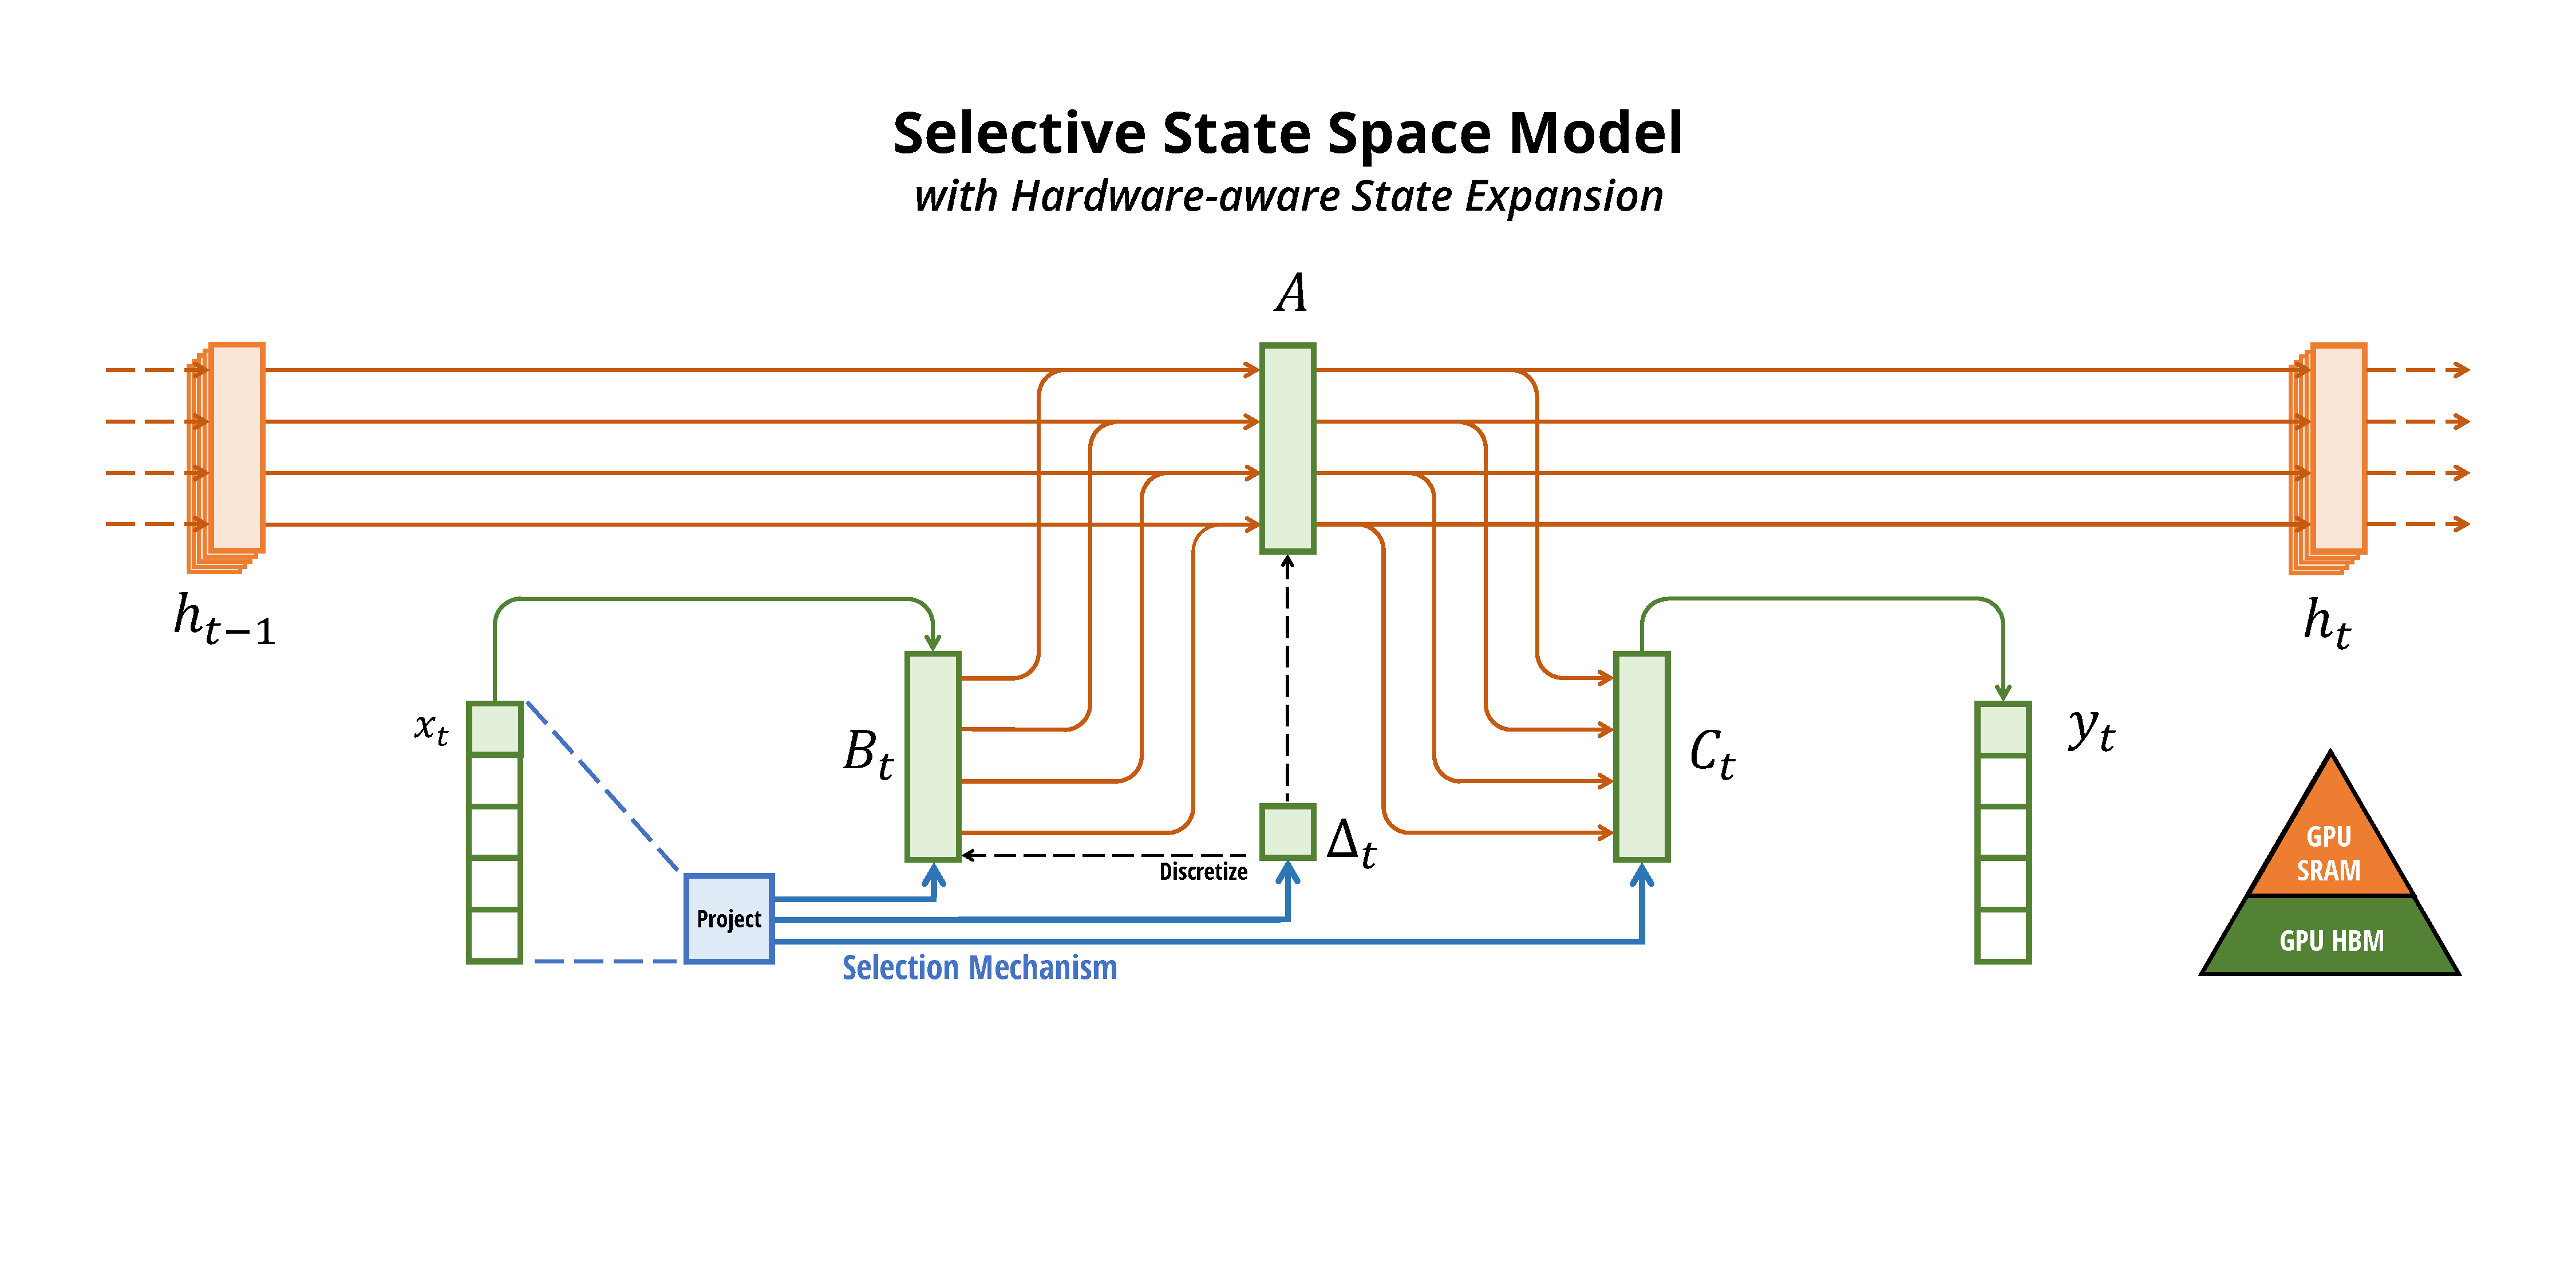
\includegraphics[width=0.9\linewidth]{mamba-fig01-selective-ssm.pdf}
  \caption[Selective state-space model with input-dependent parameters]{Selective
  state-space model: a selection mechanism makes the SSM parameters depend on
  the input. \source{Gu and Dao (2023)~\cite{gu2023mamba}, Fig.~1}}
  \label{fig:mamba-selective}
\end{figure}

\section{Hybrid Mamba--Transformer Models}

If Mamba is efficient but forgetful and attention is precise but expensive,
the natural step is to mix them. Jamba~\cite{lieber2024jamba} was the first
large model to interleave Transformer and Mamba layers with MoE
(Figure~\ref{fig:jamba}), supporting 256K-token contexts on a single 80\,GB
GPU.

\begin{figure}[!htbp]
  \centering
  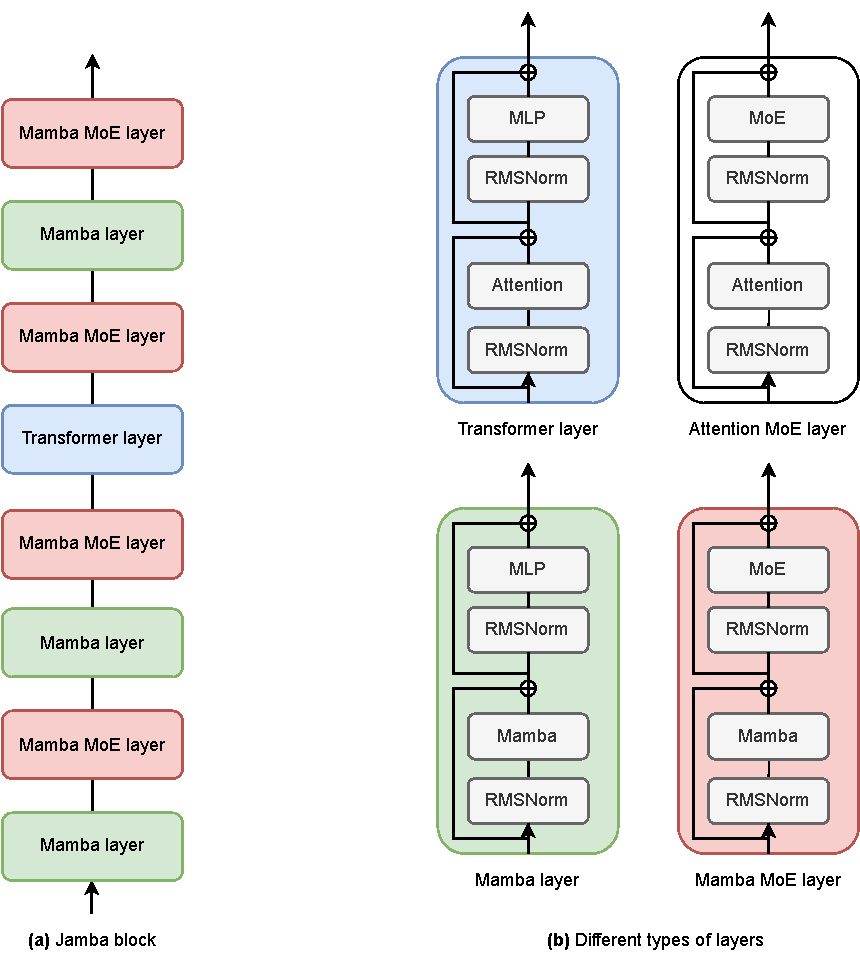
\includegraphics[width=0.5\linewidth]{jamba-fig01-block.pdf}
  \caption[A Jamba block mixing attention, Mamba and MoE layers]{(a) A Jamba
  block and (b) its layer types. \source{Lieber et al.\
  (2024)~\cite{lieber2024jamba}, Fig.~1}}
  \label{fig:jamba}
\end{figure}

Waleffe et al.~\cite{waleffe2024empirical} trained 8B Mamba, Mamba-2 and
Transformer models on the same data. Pure SSMs lagged on copying and
in-context learning tasks such as five-shot MMLU, but a hybrid of 43\%
Mamba-2, 7\% attention and 50\% MLP layers beat the Transformer on all twelve
tasks evaluated and was predicted to be up to 8$\times$ faster at generation.
Validation loss was lowest with only about 8\% attention layers
(Figure~\ref{fig:attn-ratio}): \emph{a few attention layers are enough}.

\begin{figure}[!htbp]
  \centering
  \begin{subfigure}[b]{0.44\linewidth}
    \centering
    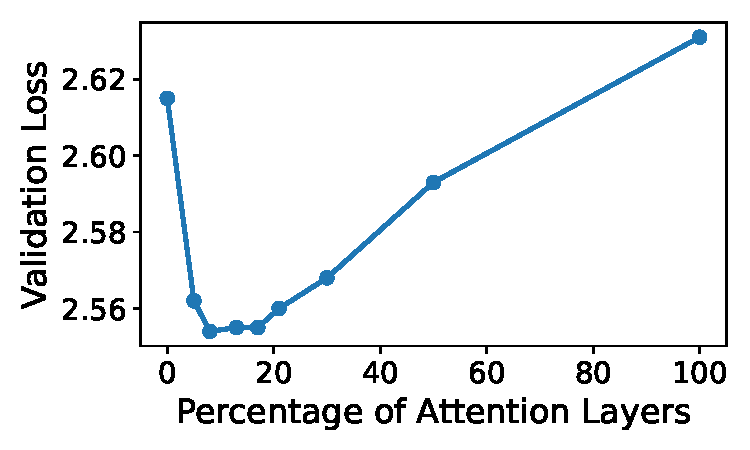
\includegraphics[width=\linewidth]{empirical-fig04-attention-ratio.pdf}
    \caption{Validation loss against percentage of attention layers.}
  \end{subfigure}\hfill
  \begin{subfigure}[b]{0.46\linewidth}
    \centering
    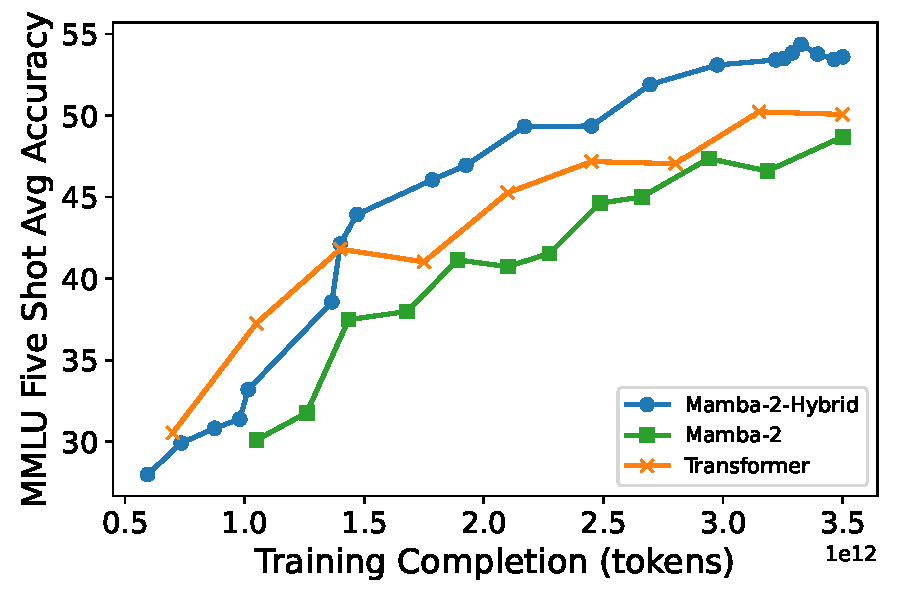
\includegraphics[width=\linewidth]{empirical-fig06-mmlu.pdf}
    \caption{Five-shot MMLU of 8B models during training.}
  \end{subfigure}
  \caption[How much attention a hybrid model needs]{How much attention a hybrid
  needs, and what it buys. \source{Waleffe et al.\
  (2024)~\cite{waleffe2024empirical}, Figs.~4 and~6}}
  \label{fig:attn-ratio}
\end{figure}

\section{The Nemotron Lineage}

\emph{Nemotron-H}~\cite{nvidia2025nemotronh} turned this finding into 8B and
56B models with about 8\% evenly dispersed attention layers
(Figure~\ref{fig:nemotronh}), matching Qwen-2.5 and Llama-3.1 while being up to
3$\times$ faster. \emph{Nemotron Nano~2}~\cite{nvidia2025nano2} applied it to a
reasoning model with up to 6$\times$ the throughput of Qwen3-8B.
\emph{\NN}~\cite{nvidia2025nano3}, the first Nemotron~3
model~\cite{nvidia2025nemotron3}, added MoE (31.6B total, 3.2B active) and
reached up to 3.3$\times$ the throughput of similar models
(Figure~\ref{fig:nano3}), but used a standard MoE and BF16 training.

\begin{figure}[!htbp]
  \centering
  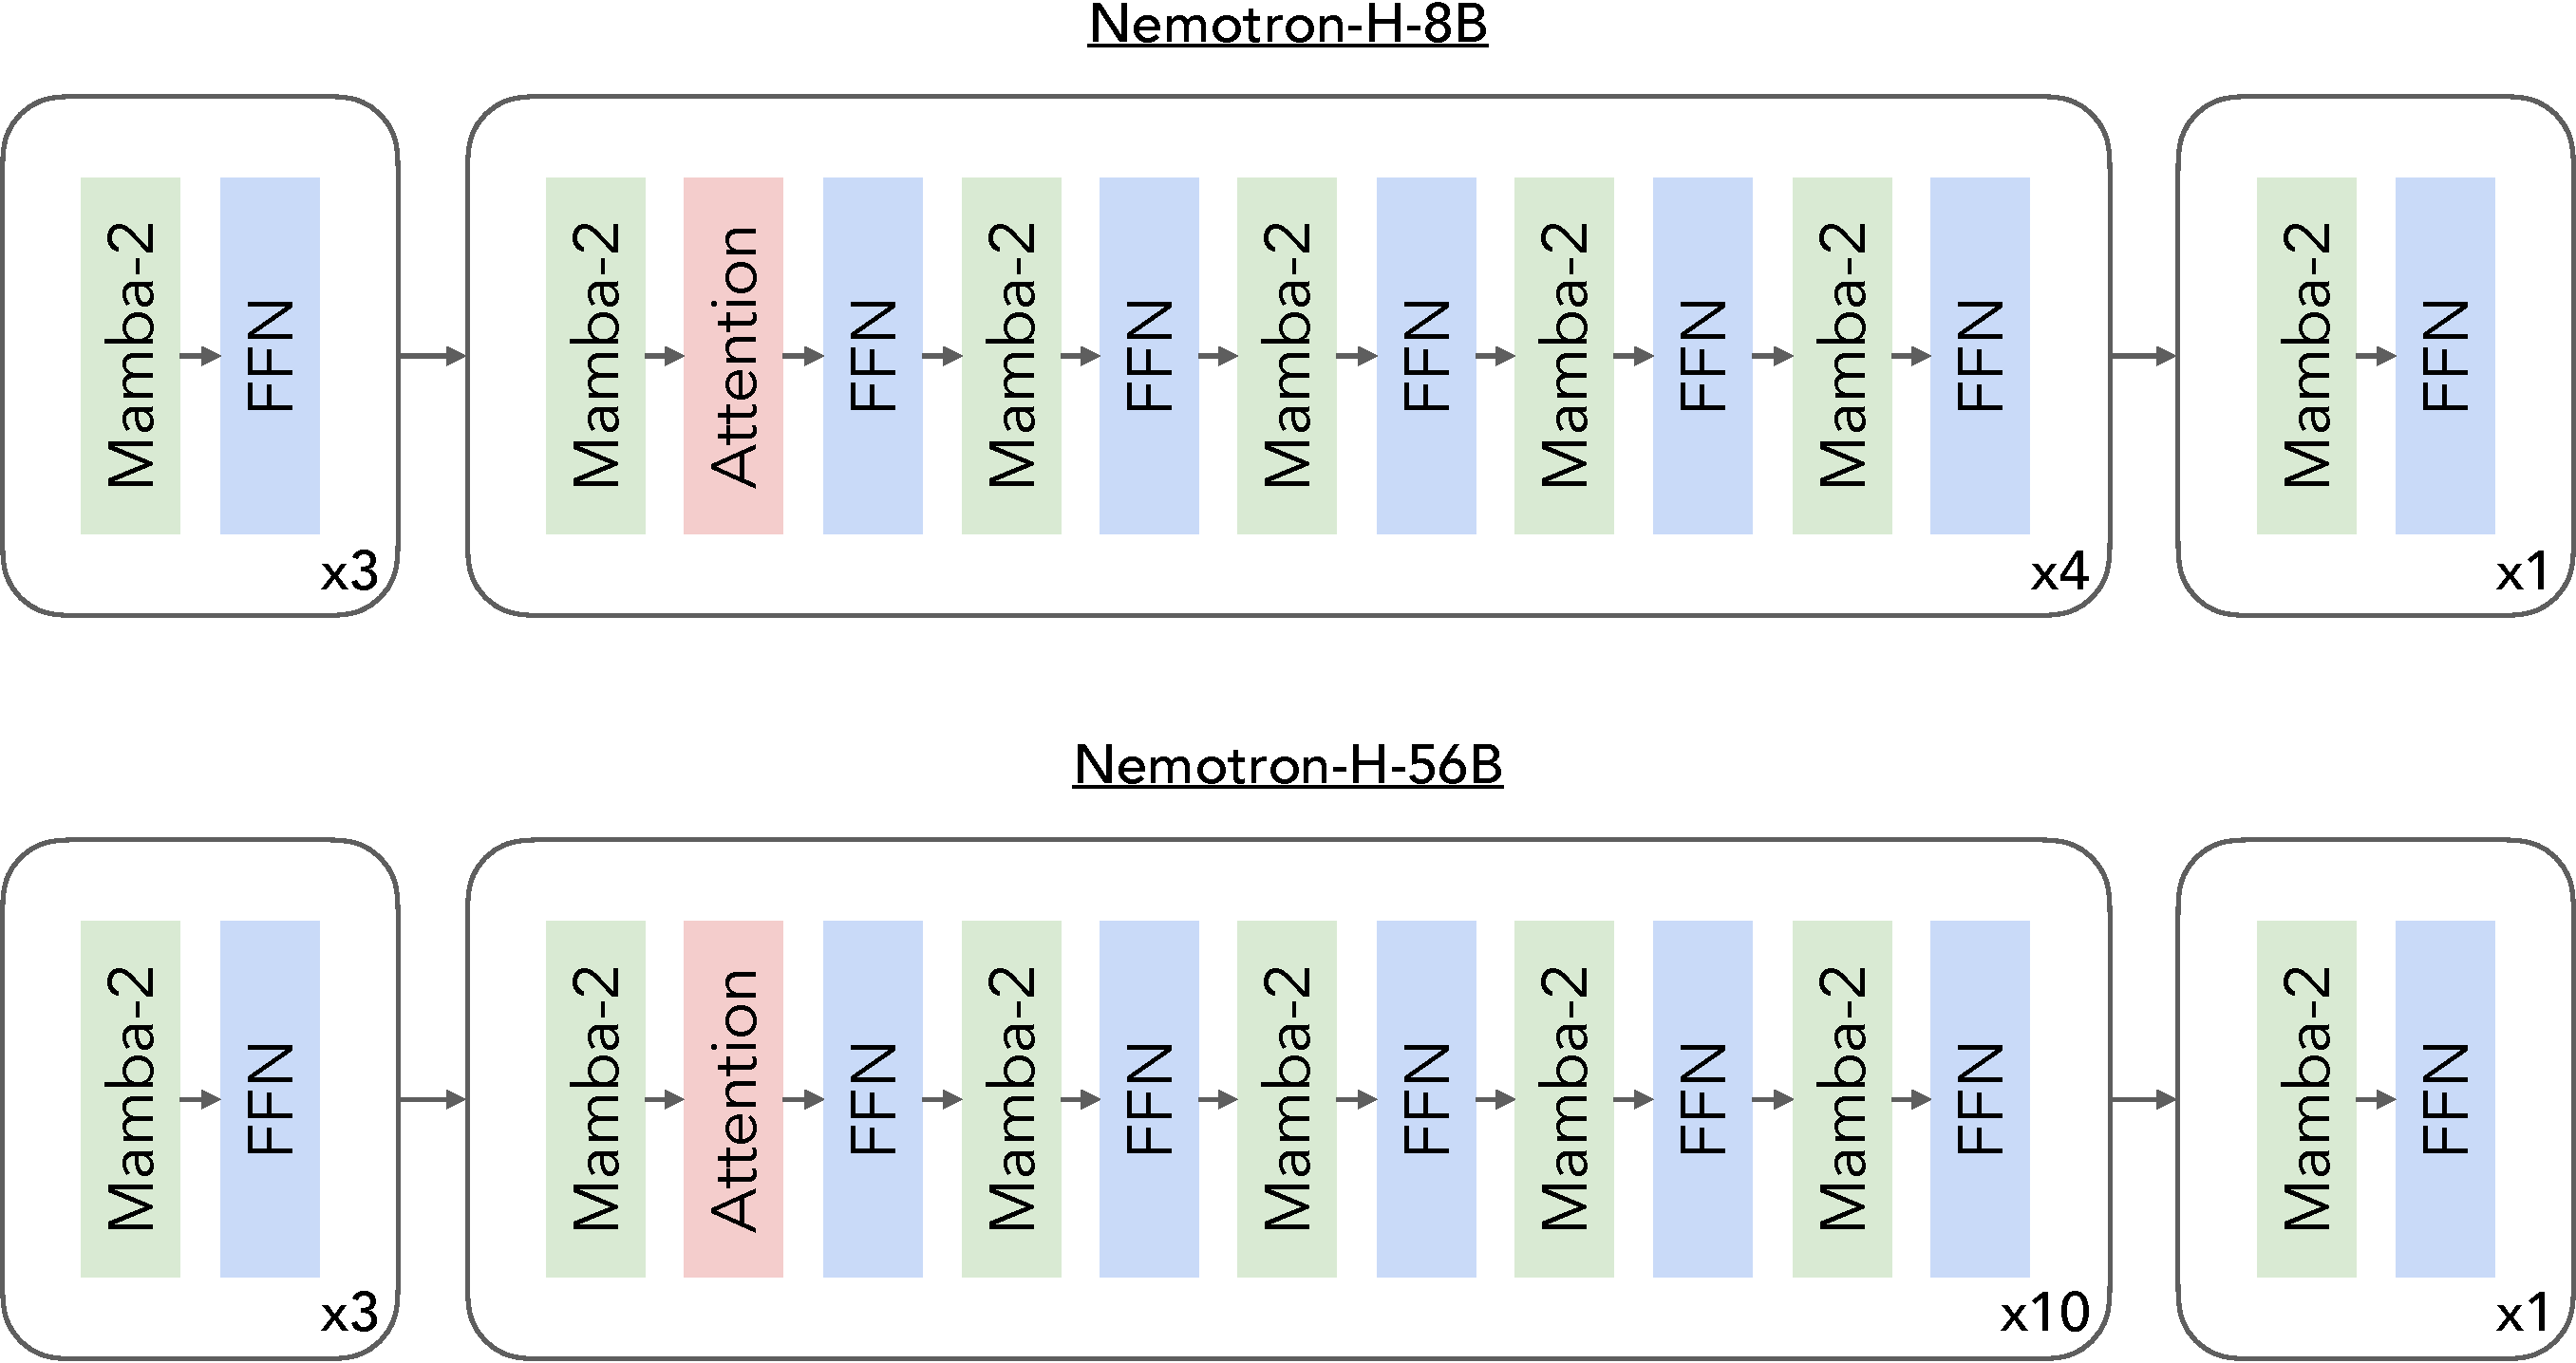
\includegraphics[width=0.8\linewidth]{nemotronh-fig02-layer-pattern.pdf}\\[4pt]
  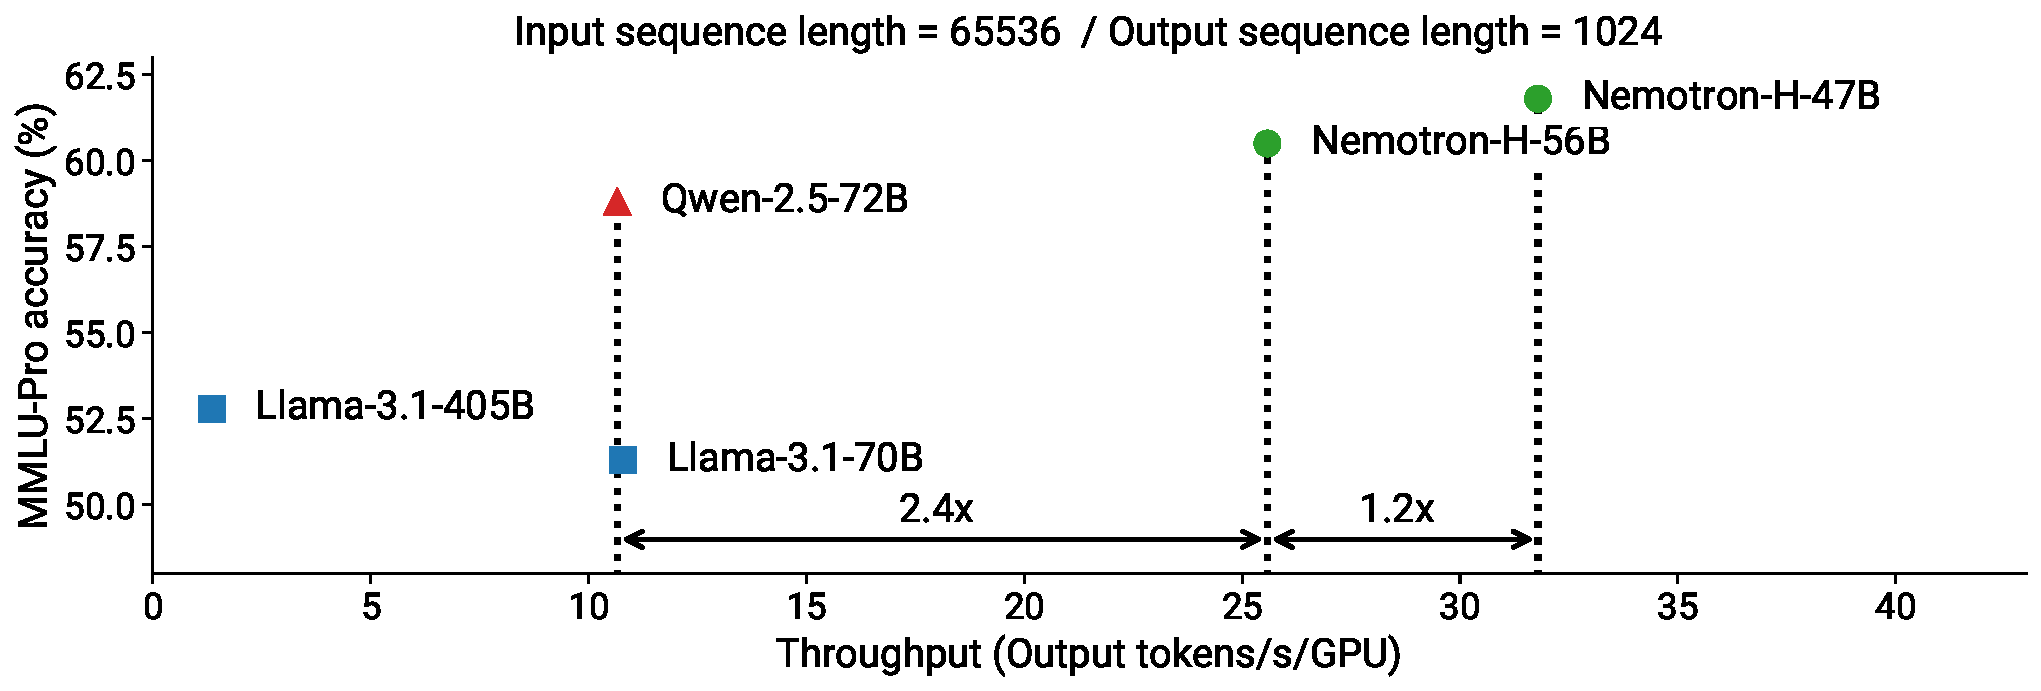
\includegraphics[width=0.8\linewidth]{nemotronh-fig01-throughput.pdf}
  \caption[Nemotron-H layer pattern and accuracy versus throughput]{Top:
  Nemotron-H layer patterns. Bottom: MMLU-Pro accuracy against inference
  throughput. \source{NVIDIA (2025)~\cite{nvidia2025nemotronh}, Figs.~2 and~1}}
  \label{fig:nemotronh}
\end{figure}

\begin{figure}[!htbp]
  \centering
  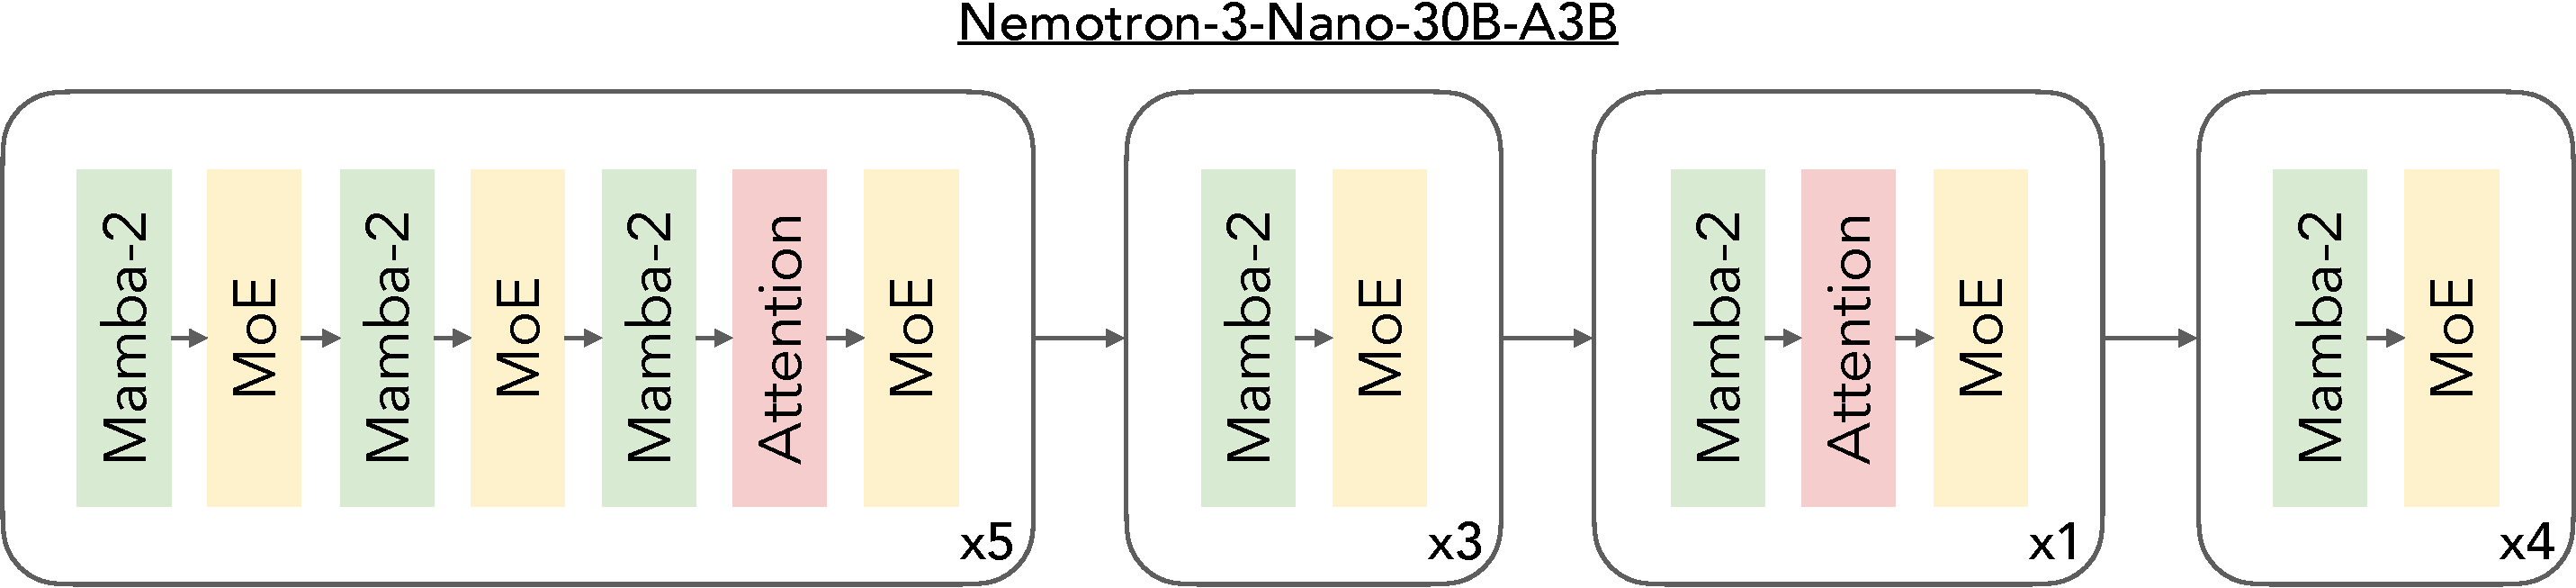
\includegraphics[width=0.78\linewidth]{nano3-fig02-layer-pattern.pdf}\\[4pt]
  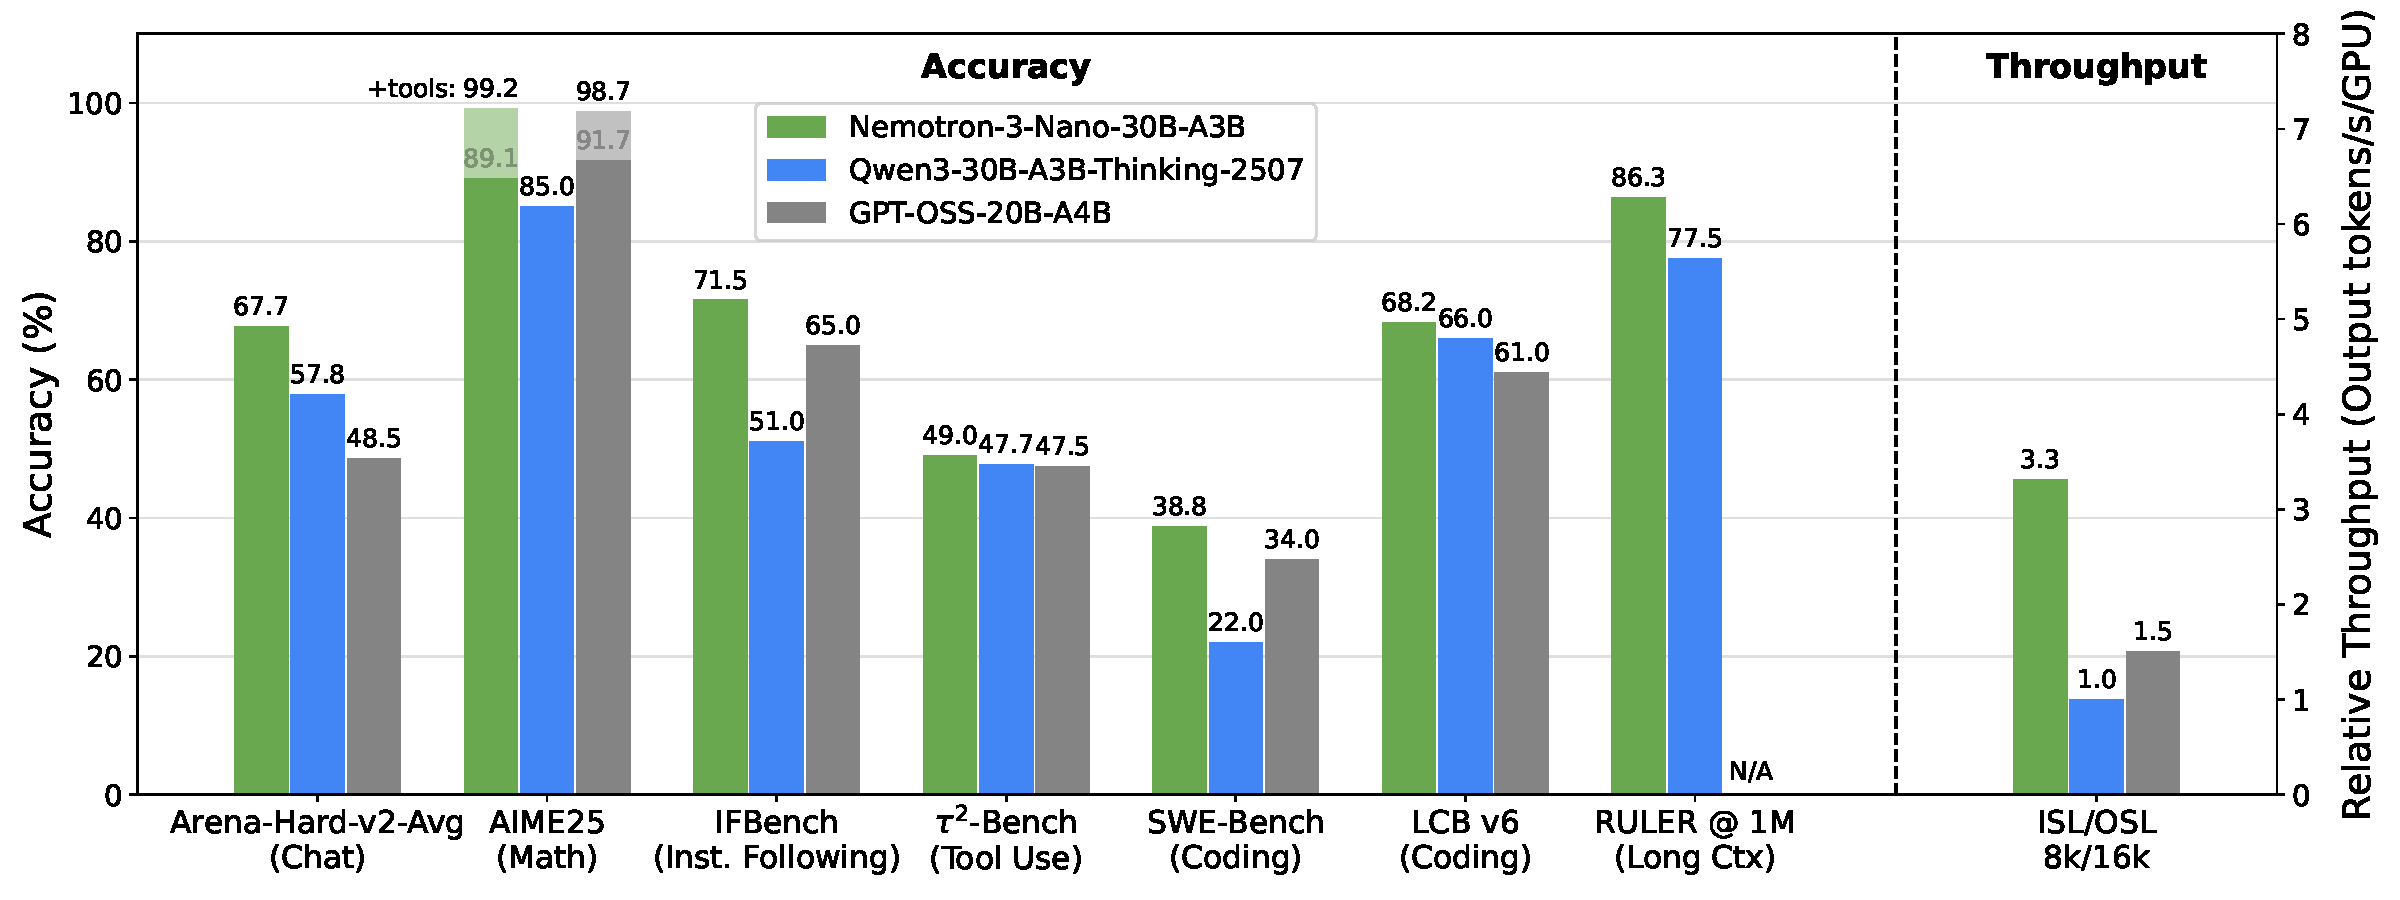
\includegraphics[width=0.88\linewidth]{nano3-fig01-accuracy-throughput.pdf}
  \caption[Nemotron 3 Nano layer pattern and accuracy/throughput comparison]{Top:
  \NN\ layer pattern. Bottom: accuracy and throughput against Qwen3-30B-A3B and
  GPT-OSS-20B. \source{NVIDIA (2025)~\cite{nvidia2025nano3}, Figs.~2 and~1}}
  \label{fig:nano3}
\end{figure}

\section{Supporting Techniques}

\textbf{Mixture-of-Experts.} The sparsely-gated MoE~\cite{shazeer2017moe} was
scaled by GShard~\cite{lepikhin2020gshard} and refined by
DeepSeek-V3~\cite{deepseek2024v3} with fine-grained experts and
auxiliary-loss-free balancing. LatentMoE~\cite{elango2026latentmoe} moves the
experts into a lower-dimensional latent space and is used in \NS.

\textbf{Multi-token prediction.} Gloeckle et al.~\cite{gloeckle2024mtp}
trained models to predict several future tokens with extra heads on a shared
trunk (Figure~\ref{fig:mtp-meta}), which pairs naturally with speculative
decoding~\cite{leviathan2022speculative,chen2023speculative}.

\textbf{Low-precision training.} NVFP4~\cite{nvidia2025nvfp4} showed stable
4-bit pretraining of a 12B model over 10 trillion tokens.

\begin{figure}[!htbp]
  \centering
  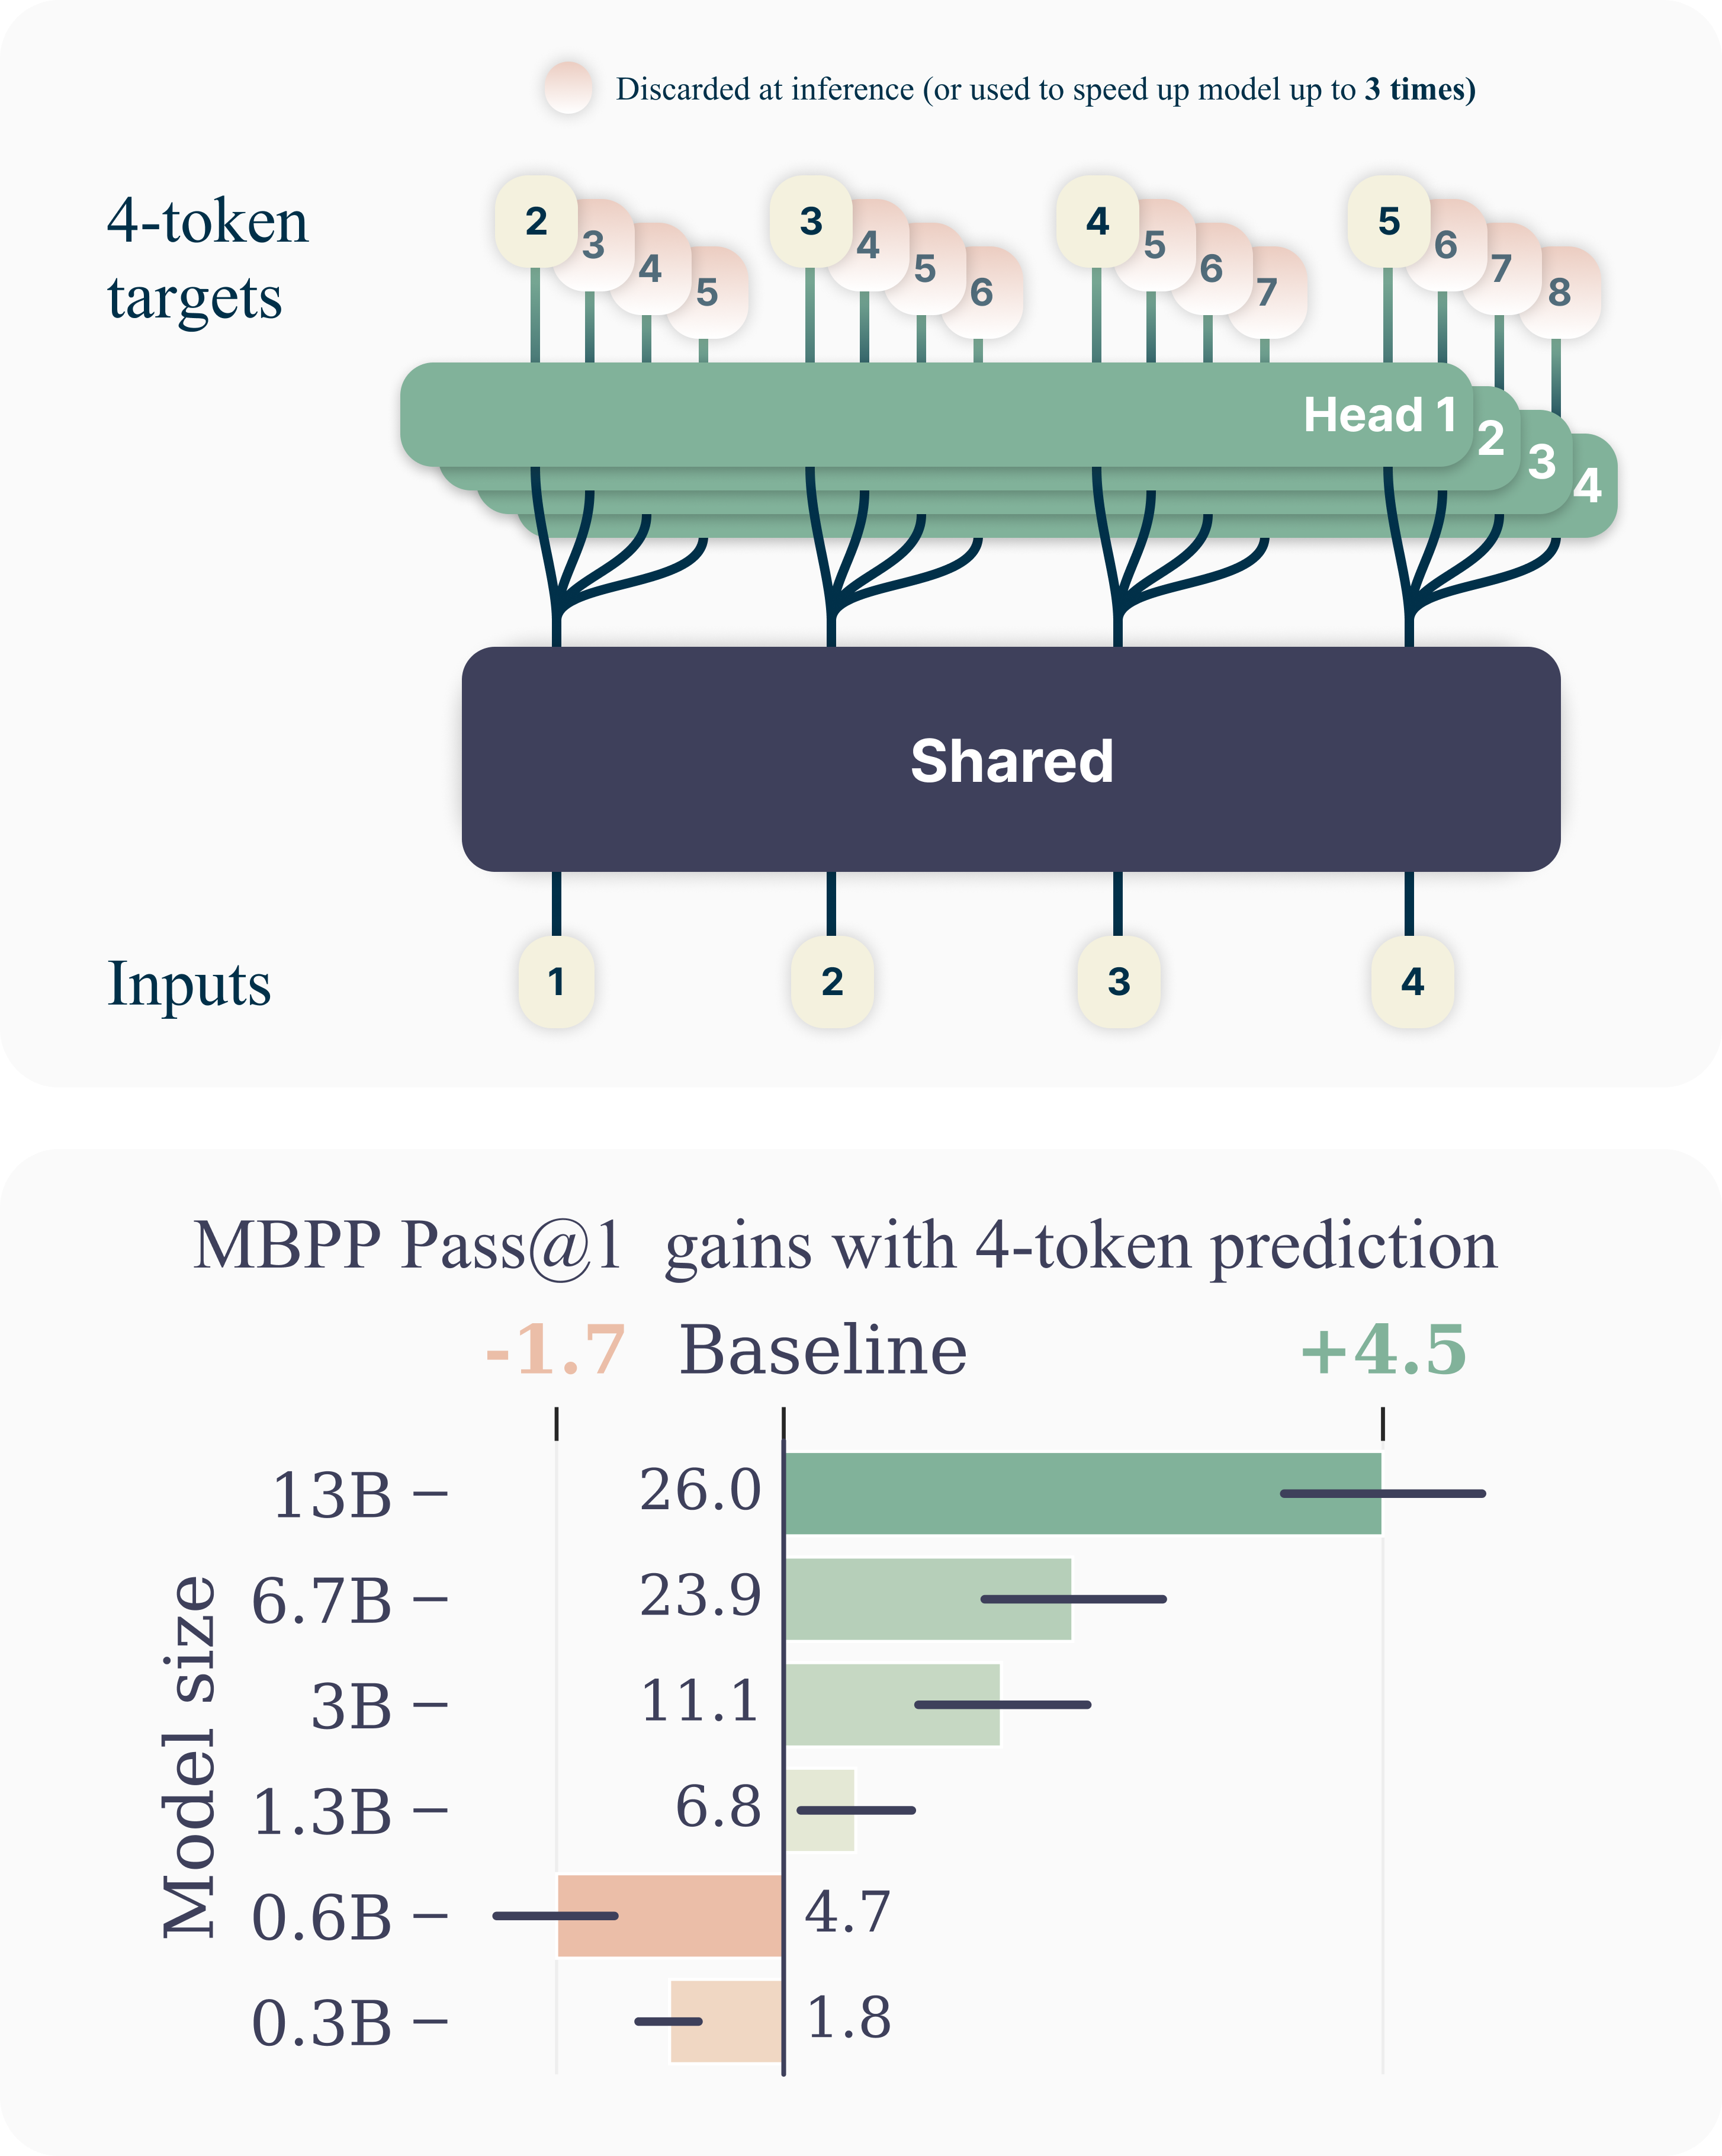
\includegraphics[width=0.48\linewidth]{mtp-fig01-overview.png}
  \caption[Multi-token prediction with several output heads on a shared trunk]{Multi-token
  prediction with several output heads on a shared trunk.
  \source{Gloeckle et al.\ (2024)~\cite{gloeckle2024mtp}, Fig.~1}}
  \label{fig:mtp-meta}
\end{figure}

\section{Summary of the Survey}

Table~\ref{tab:survey} summarises the main works and the gap each leaves open.

\begin{table}[!htbp]
\centering
\small
\caption{Summary of the literature survey}
\label{tab:survey}
\begin{tabularx}{\linewidth}{@{}P{3.0cm}LL@{}}
\toprule
\textbf{Study} & \textbf{Main contribution} & \textbf{Limitation / gap} \\
\midrule
Vaswani et al.\ (2017) \cite{vaswani2017attention} &
Transformer built on self-attention. &
Quadratic compute; KV cache grows with context. \\
Gu and Dao (2023) \cite{gu2023mamba} &
Mamba: selective, linear-time SSM. &
Fixed-size state; small to medium scale. \\
Dao and Gu (2024) \cite{dao2024mamba2} &
Mamba-2 and SSD; 2--8$\times$ faster layer. &
State is a lossy summary. \\
Lieber et al.\ (2024) \cite{lieber2024jamba} &
Jamba: first large hybrid with MoE. &
One fixed ratio; standard MoE. \\
Waleffe et al.\ (2024) \cite{waleffe2024empirical} &
Hybrid with $\sim$8\% attention beats a Transformer. &
Dense models only. \\
NVIDIA (2025) \cite{nvidia2025nano3} &
\NN: hybrid plus MoE at 30B. &
Small scale; standard MoE, BF16. \\
NVIDIA (2026) \cite{nvidia2026super} &
\NS: 120B with LatentMoE, MTP and NVFP4. &
Large memory; trails Qwen3.5 on some tasks. \\
\bottomrule
\end{tabularx}
\end{table}

\section{Research Gap}

The survey shows a clear progression. Mamba and Mamba-2 solved the cost of
long sequences but lost exact recall; Jamba and the empirical study of Waleffe
et al.\ showed that a small share of attention restores it; and the Nemotron-H,
Nano~2 and \NN\ models proved the idea in practice up to about 30 billion
parameters. What remained open was whether such a hybrid could be scaled to
more than one hundred billion parameters, combined with a hardware-aware MoE,
trained in 4-bit precision and post-trained for demanding agentic tasks while
staying competitive with the best Transformers. \NS\ is the first open model
to attempt all of these together, which is why it was chosen for this seminar.
